\chapter{Installation and first script}

In this chapter we will explain how to install the motoman project on your computer and make you write a script that use a motion planner to find a plan for the robot. This chapter is essentially a chain of instructions, there are few details about the files you will manipulate. The next chapter will be more in depth.

\section{Initialization}
First thing to do is to create a ROS workspace where you will work.  So go to where you want to create your workspace and then create the workspace with a \emph{src} folder inside. Then go inside the \emph{src} folder and initialize the catkin workspace.

\begin{lstlisting}
cd /where/you/want/your/workspace
mkdir -p my_workspace/src
cd my_workspace/src
catkin_init_workspace
\end{lstlisting}

Then download the motoman project repository. To do it you need to have the git program in your computer. To install git just type the following command.

\begin{lstlisting}
sudo apt-get install git
\end{lstlisting}

Then you need to download the repository. The \emph{clone} command after the \emph{git} command means you want to take the repository data and copy them into your current folder. So first go where your ros workspace and clone the github repository inside the \emph{src} folder.  

\begin{lstlisting}
cd my_workspace/src
git clone https://github.com/Nishida-Lab/motoman_project.git
\end{lstlisting}

Then normaly a \emph{motoman\_project} file would have been created in your \emph{src} folder. The next step is to actually compile the project. To do this you need to use the \emph{catkin\_make} command in the root of your workspace. But before that you need to be sure to have all the dependencies. 


\begin{lstlisting}
cd my_workspace
wstool init src src/motoman_project/dependencies.rosinstall
sudo apt-get install ros-indigo-industrial-msgs
sudo apt-get install ros-indigo-industrial-robot-simulator
sudo apt-get install ros-indigo-industrial-robot-client
sudo apt-get install ros-indigo-ros-controllers
rosdep install -i --from-paths src
catkin_make
\end{lstlisting}

After compiling everything (it could take some time!) you will be able to use the project. A simple test is to launch one of the launch file of the project. First you need to source the workspace to be sure that you can use the ROS command associated to your project.

\begin{lstlisting}
cd workspace
source devel/setup.bash
\end{lstlisting}

Then launch the empty environment with motoman inside by the following command.

\begin{lstlisting}
cd my_workspace
source devel/setup.bash
roslaunch motoman_gazebo sia5_empty_world.launch
\end{lstlisting}
\begin{figure}
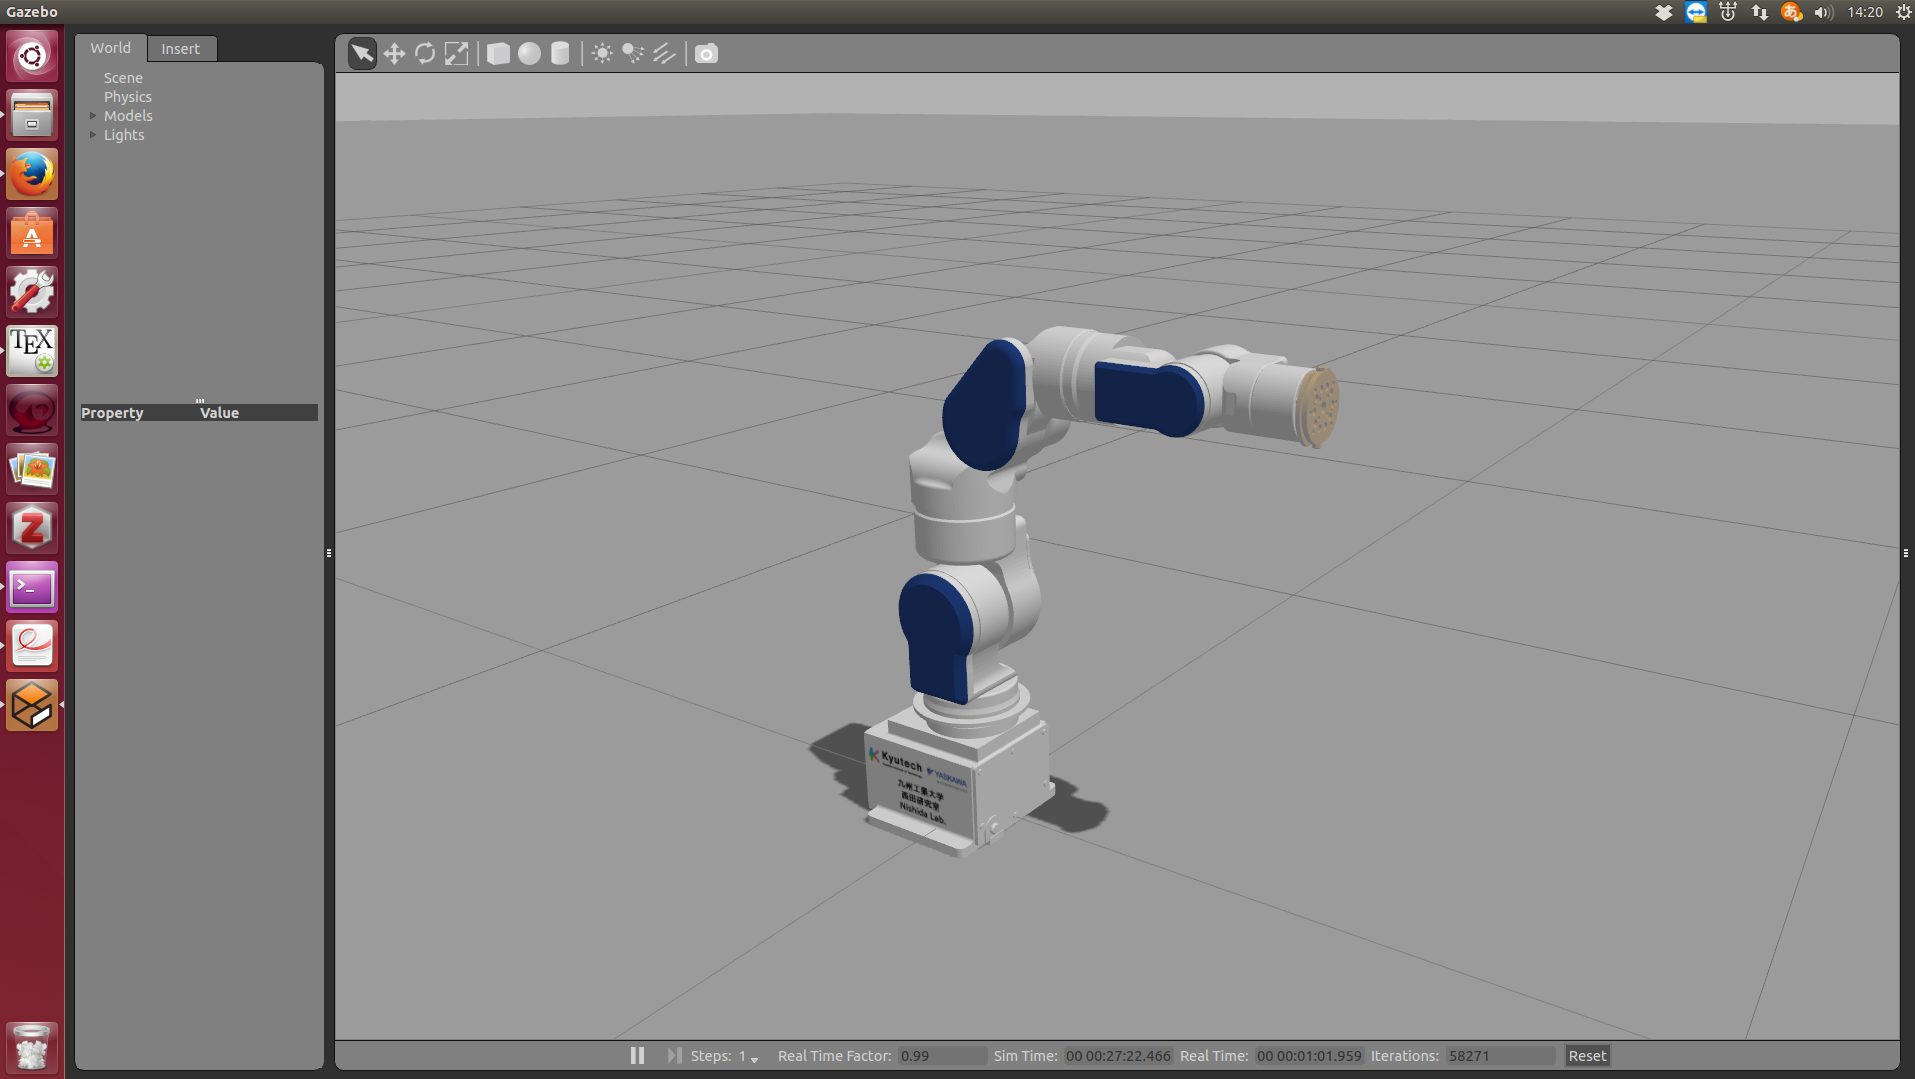
\includegraphics[scale=0.132]{images/installation_first/launch_gazebo.png}
\centering
\caption{That is what you should see if the installation has been rightly completed.}
\label{fig:launch_gazebo}
\end{figure}
You should normally have the gazebo software begin to run and you can soon see the motoman robot sia5 inside your screen like in Figure \ref{fig:launch_gazebo}.

\section{Finding a motion plan}

In this section we will create a script that connect to the robot and use a motion planner to find a plan between a start position and a goal position. There are many things to do before being able to do it but if you follow the steps it should not be difficult. This section focus on writing the script rather than understanding everything. The next chapters will give more details about it.

To begin everything we need to create a ros package where our script will be written. You normally have one metapackage in your \emph{src} folder named \emph{motoman\_project}. It is really easy to create a new package in ros with the catkin command. You can name it anything you want, in this manual we will call it \emph{motion\_planning}. To make our script able to run we will need to initialize gazebo and rviz. For this reason you will need to launch gazebo and rviz every time you will want to use your script. As it is tiring it is easier to just create a launch file that will be launch before the script and that will automatically call the gazebo and rviz part by itself.


\begin{lstlisting}
cd workspace/src
catkin_create_pkg motion_planning roscpp
cd motion_planning
mkdir launch
cd launch
touch initialization.launch
\end{lstlisting}

We use the \emph{roscpp} argument because our package will need it to create a ros node. You can create the following launch file in the launch folder, we will describe it more later. 

\lstinputlisting[caption=initialization.launch]{code_files/installation_first/initialization.launch}


In the \emph{src} folder we can write our script to move the robot. First we create the file (we named it \emph{moving.cpp} but every name is ok, just change the CMakeLists file accordingly). 

\begin{lstlisting}
cd workspace/src/motion_planning/src
touch moving.cpp
\end{lstlisting}

Then just write the following code inside the \emph{moving.cpp} file. This script shows how to ask moveit to find a plan from the current position to any goal position you define. However it may be possible that no plan will be found. In this situation the workspace is empty so it should be quite easy to find a solution but when a lot of obstacles are populating the environment then it becomes a difficult task to find a collision free trajectory for the robot.

\lstinputlisting[language=c++,caption=moving.cpp]{code_files/installation_first/moving.cpp}

After having wrote the script we need to compile it. To do it we need to modify two files : the CMakeLists.txt and package.xml. These two files have already been created when you created the package with the catkin command, so you just have to replace their contents with the following files.

\lstinputlisting[caption=CMakeLists.txt]{code_files/installation_first/CMakeLists.txt}

\lstinputlisting[caption=package.xml]{code_files/installation_first/package.xml}


So now everything have been done to use the script you wrote. First compile everything. Every time you will modify your C++ files you will need to compile again all your workspace. Once compile you will need to first launch the launch file that will initialize gazebo and rviz, it will also load the ompl library. When the launch file has been ran you can then run your script.


\begin{lstlisting}
cd workspace
catkin_make
source devel/setup.bash
roslaunch motion_planning initialization.launch
rosrun motion_planning motion_planning
\end{lstlisting}


The result of this script could be seen in Figure \ref{fig:simple_moving}. The figure shows a trail of the movement. You can activate it by clicking on the left panel to the \emph{motion planning} line and then clicking on the \emph{Show trail} box as it can be seen in the Figure \ref{fig:show_trail}.  

\begin{figure}
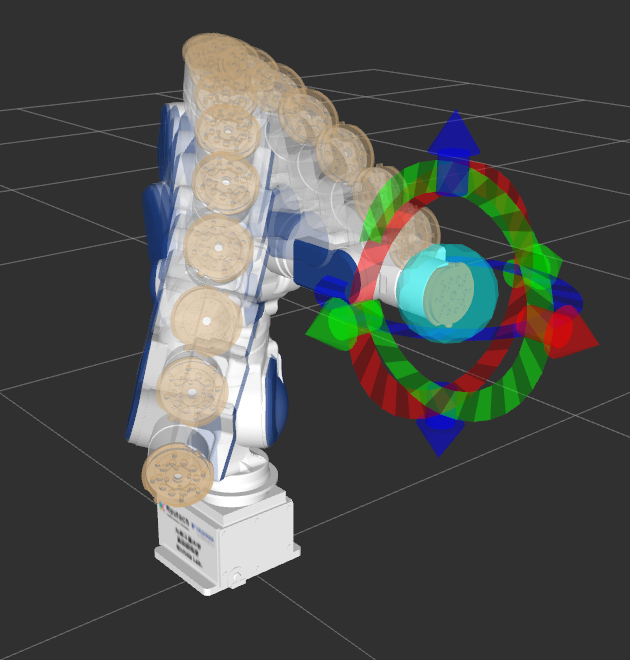
\includegraphics[width=8cm]{images/installation_first/simple_moving.png}
\centering
\caption{Yo}
\label{fig:simple_moving}
\end{figure}



\begin{figure}
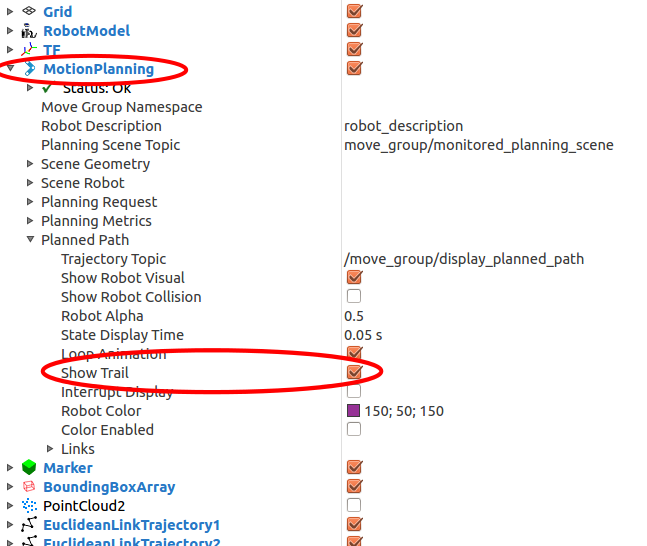
\includegraphics[width=8cm]{images/installation_first/show_trail.png}
\centering
\caption{Yo}
\label{fig:show_trail}
\end{figure}